\subsubsection{Setup}
    This test has been performed on actual data used by Axpo.
    The view selected contains forecasts from multiple providers related to multiple categories.
    It has been chosen since it is one of the largest and slowest tables used by the company.
    The view contains 106 million rows.
    
    \paragraph{Materialization}
        Executing tests on a view would have produce inaccurate results, since multiple operations (mostly joins with dimensional table) are performed each time.
        To avoid this problem, the data has been copied to a separate table, created appositely for testing.
        
        In this way, we also made sure no one else would use this table while the tests were being executed.
        
    \paragraph{Excessive table size}
        The size of the table was still however excessive for some tests; the two main problems encountered were:
        \begin{itemize}
            \item Excessive computational times
            \item Not enough RAM to store the results
        \end{itemize}
        
        The first issue prevented running an appropriate number of tests, since a single query execution could take more than half a day.
        It was necessary to perform multiple runs of each query to obtain more reliable results, so each test would have taken several days.
        
        The second problem was related to the PC used for executing the tests: asking to retrieve a huge number of rows would have required a very large amount of RAM on the machine to temporarily store the results.
        Since the machine was limited to 8GB RAM, it often encountered \textit{Out of Memory} errors, which prevented the tests from completing.
        
        As a consequence, I decided to leave only the most recent 10 million records, and perform the tests on this smaller set.
        Since all data in the original table is updated daily, taking the last \textit{n} days leaves all the value distributions intact.
        
\subsubsection{Results}
    The execution times measured from the queries mostly confirmed the results obtained from the metrics.

    \begin{figure}[p]
        \centering
        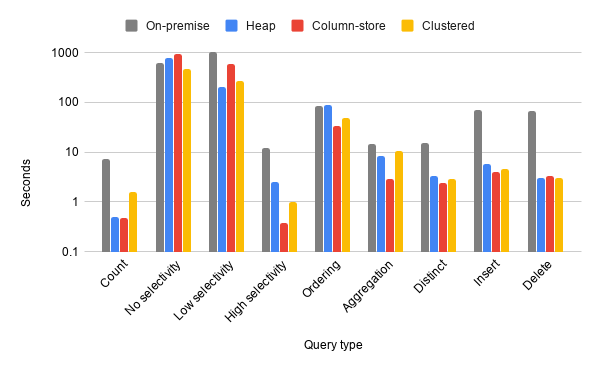
\includegraphics[width=\textwidth]{res/tests/perf_queries.png}
        \caption{Query execution times for both databases. Different table options have been tested.}
        \label{fig:tests:perf:queries:results}
    \end{figure}
    
    \begin{figure}[p]
        \centering
        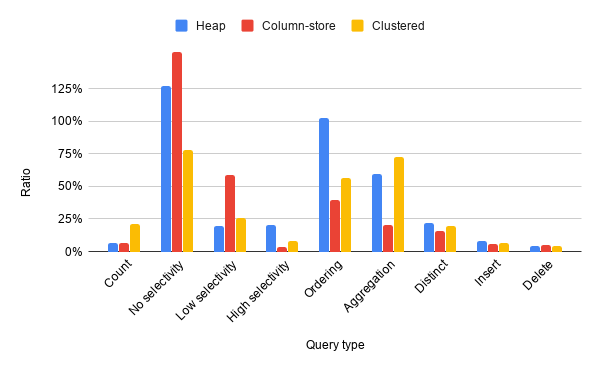
\includegraphics[width=\textwidth]{res/tests/perf_queries_perc.png}
        \caption{Execution time ratio between Data Warehouse and on-premise database, for each query type.}
        \label{fig:tests:perf:queries:results:ratio}
    \end{figure}
    
    The times obtained are shown in Figure \ref{fig:tests:perf:queries:results}.
    
    Figure \ref{fig:tests:perf:queries:results:ratio} shows the execution time ratio between the Data Warehouse and the on-premise database, for each query type.
    
    \paragraph{Initial considerations}
        As we can see, the Data Warehouse performs better than the on-premise database on almost all test cases.
        
        Count operations, as well as insertions and deletions can be computed in a very short amount of time, especially when compared to the on-premise database.
        
        Selection operations, on the other hand, are directly dependant on the selectivity degree of the query.
        A very selective query is very performing, while a completely non-selective query (such as \code{SELECT * FROM <table>}) is even outperformed by the on-premise database.
        
        All the other operations are generally more performing than the on-premise database, but their performance is strictly related to the table type.
        
    \paragraph{Heap tables}
        Heap tables present the lowest execution time for deletion operations, and a very low time for insertions.
        This is because of the structure of heap tables, which don't need to update any index when or removing data from a table.
    
        Ordering operations, however, perform poorly, since this table structure stores the values in unsorted order.
        As a consequence, each page needs to be accessed multiple times to sort all values.
        
    \paragraph{Column-store tables}
        Column-store tables are the fastest option for high-selectivity queries, as well as aggregation and duplicate removal operations.
        
        Since data is stored in column format, selection operations on specific attributes can be performed directly on the column, without retrieving unneeded data.
        
        The same principle applies to aggregation and duplicate removal: the columns necessary for the operation are stored in the same memory blocks, decreasing the amount of read operations needed to compute the result.
        
        On the other hand, low-selectivity queries are penalized, since the particular column structure created an additional reading overhead when multiple columns are required for a lot of records.
        
    \paragraph{Clustered tables}
        Clustered tables offer the best performance overall, although they are very dependant on the workload.
        
        For instance, we can notice that the aggregation operation, which has not been performed on the clustering index, performs poorly.
        
        As a consequence, this table is a very good choice if most operations have conditions on the same attributes.
        
\subsubsection{Considerations}
    From the results, it is clear that the Data Warehouse offers higher performances than the on-premise database.
    
    Insertion and deletion operations are very efficient on all table formats, while other operations are dependent on the attributes present in the query, as well as the table format chosen.
    
    There is, however, no general solution.
    As we have shown, for example, a column-store table can be very efficient on operations requiring access to a small number of attributes, but can be outperformed even by the on-premise database if a large number of columns and rows is requested.
    
    As a consequence, it is always important to keep in mind the workload when creating a table.
    Choosing the wrong option can worsen performance, in the worst cases making the Data Warehouse even slower than a local database.
    
    On the other hand, if the right choices are made, users can notice a large improvement in execution speed, up to 33 times in the best scenario (a high-selectivity query on a column-store table).
    
